\chapter{Synchronization System Case Study}
\etocsettocstyle{\rule{\textwidth}{1pt}}{\rule{\textwidth}{1pt}} % style for toc
\localtableofcontents
\label{chap:synchronization}

In eCommerce, synchronization systems are often needed to ensure that the online store reflects the current state of the store's products' logistics. Brick-and-mortar stores manage their inventory with logistical software system. A synchronization system that ensures the consistency and truthfulness of the online store is crucial.
The main focus of this chapter is on a practical comparison between serverless and monolithic implementations of such a synchronization system. Synthetic workloads are generated and two mock servers, simulating a logistics system and a Shopify store are used.

\section{System Overview}

The synchronization system is designed to maintain a consistent state between the store's logistics system and the Shopify store. It ensures that for every Item on PS, there exists an equivalent Variant on SH and that it is up-to-date, with PS being the source of truth. The synchronization task is mainly encapsulated in a single function, \texttt{syncModel(modelCode: String)}, which is deployed as an action on OpenWhisk in the serverless implementation and exposed as a route in the monolithic version.

API clients encapsulate CRUD operations for PS and SH. They handle operations such as fetching and updating items or stocks on PS and managing products, variants, and stocks on SH. 

\section{Experimental Setup}

The experimental setup involved deploying the monolithic and serverless implementations on machines of type m510 on CloudLab in the Utah cluster. Benchmarks were conducted using increasing workloads to assess the performance of each system. A custom-built rate limiter was used to control the flow of requests to the systems.

\section{Benchmarking Process}

This section describes the workload and the main components involved in the benchmarking process. It also explains the methodology used in benchmarking the serverless and monolithic implementations.

\subsection{Main Components}

\subsubsection{PS Server}
The PS Server contains items and their stock count as shown in the following structures:

\begin{minted}{swift}
struct PSItem: Identifiable {
    ...
    let itemCode: String
    let modelCode: String
    var id: String { itemCode }
    ...
}

struct PSStock: Identifiable {
    let itemCode: String
    var id: String { itemCode }
    var stock: Int
}
\end{minted}

Many \textit{Items} belong to one \textit{Model}. A \texttt{PSItem} is identified by its \texttt{itemCode}, and a model is identified by a \texttt{modelCode}.

\subsubsection{SH Server}
The SH Server contains products and their stock count as shown in the following structures:

\begin{minted}{swift}
struct InventoryLevel: Identifiable {
    let inventoryItemID: Int
    var id: Int { inventoryItemID }
    var stock: Int
}

struct SHVariant: Identifiable {
    let id: Int
    let productID: Int
    let sku: String
    let inventoryItemID: Int
}

struct SHProduct: Identifiable {
    let id: Int
    let handle: String
    ...
    let variants: [SHVariant]
}
\end{minted}

\subsubsection{ModelSyncer}
A \textit{Model} from the PS Server corresponds to an \texttt{SHProduct} from the SH Server. A \textit{Model}'s \texttt{PSItem}s correspond to the respective \texttt{SHProduct}'s \texttt{SHVariant}. A \texttt{PSItem}'s stock (\texttt{PSStock}) corresponds to the respective \texttt{SHVariant}'s \texttt{InventoryLevel}. The goal of the \texttt{ModelSyncer} is to ensure that every model from the PS Server is reflected by an equivalent product on the SH Server (including stock listings).

\subsection{Workload}
A workload can be characterized by two variables:

1. Total number of models: The total number of models that should be generated on the PS Server. For each model, a number of items are generated ranging from 1 to 20.

2. Seed: Two numbers (xSeed and ySeed) that will be used for randomization. A pseudo-random number generator (PRNG) will be seeded with these numbers and will be used for all functions concerning randomization. This ensures that given these two variables the generated resources on the two servers will always be the same. Any reference to randomness, from now on, refers to pseudo-randomness provided by the PRNG.

\subsection{Benchmarker}

The Benchmarker does three main things:

1. Setup the two servers

2. Sync all models

3. Return metrics concerning step 2. Metrics include, among other things, the time it took, memory and space usage.


\subsubsection{Setting up the servers}
The Benchmarker will be referred to as `B` to avoid repetition.

\paragraph{Generating models on PS Server}
`B` sends a GET request to PS Server at the path `/generate/modelCount/xSeed/ySeed`. The PS Server generates \texttt{modelCount} models using the \texttt{(xSeed, ySeed)} seed.

\paragraph{Generating equivalent resource on SH Server}
For each model from the PS Server, the equivalent resource on the SH Server can be in one of three states:

1. Equivalent resources exist (SHProduct, SHVariant, InventoryListing) and are up to date.

2. Equivalent resources exist partially (SHProduct, SHVariants, InventoryLevels) and are not up to date. Partially exist means some items might not have an equivalent SHVariant on the SH Server. "Not up to date" means some properties of the resource on the SH Server might need updating (source of truth is always PS Server).

3. No equivalent resources exist for that model. That model does not exist on the SH Server. Its equivalent resources (SHProduct, SHVariants, InventoryLevels) have to be created from scratch.

SH Server has initially no data. \textbf{N} = total number of models generated on PS Server. \textit{P} = number of models partially synced on SH Server (state 2). \textit{F} = number of models fully synced on SH Server (state 3).

My apologies for the abrupt cut-off. Here is the continuation of the Benchmarking Process section:

`B` randomly generates the numbers P and F given the following constraints:
* \textbf{N} $>$ 0
* \textit{P}+\textit{F} < \textbf{N}
* 0 $\le$ \textit{P} $\le$ \textbf{N}
* 0 $\le$ \textit{F} < \textbf{N}

The sum of the numbers of partially and fully synced models should not exceed the total number of models. All models could be partially synced, but all models should not be fully synced as there would be no work to be done.

`B` requests \textit{P}+\textit{F} random models from the PS Server. Then, `B` constructs the partially and fully synced products from the P and F models, respectively, along with their respective stocks. The RNG is used to generate random data such as IDs and stock counts. `B` finally sends this data to the SH Server on the route `batchProductsAndStocks`.

At this point, the two servers are set up and ready to run any benchmarks to sync any models.

\subsubsection{Running a workload}

The process of running a workload is very similar between the serverless and the monolithic implementations. The only way they differ is in the `syncModel` function. To encapsulate this behavior and simplify the benchmarking, the following protocol is defined:

\begin{minted}{swift}
protocol WorkloadRunner {
    init(psURL: URL, shURL: URL, msDelay: Int?)
    static var name: String { get }
    var psClient: MockPsClient { get }
    var shClient: MockShClient { get }
    func runSync(sourceData: SourceData) async throws -> (Int, Int, [UInt64])
}
\end{minted}

Any type that fulfills these requirements can then be used with the Benchmarker and get results.

The `runSync` function takes some source data (the current data on the two servers) and returns S, F, L where S is the number of successful syncs, F the number of failed syncs, and L is an array that contains the latency observed for each sync (the amount of time it took for a single model sync to complete).

This allows the Benchmarker to easily get comparative results for a range of workload sizes for each `RunnerType`. For instance, for a given workload, it can easily set up the servers and run an implementation (make it sync every model):

\begin{minted}{swift}
static func runOnce(workload: Workload, runner: WorkloadRunner) async throws -> (String, Duration, Int, Int, [UInt64]) {
    let name = type(of: runner).name
    print("Setting up servers for ", name)
    await setUpServers(for: workload)
    print("Retrieving source data...")
    let source = await getSourceData()
    print("Running..")
    var (successes, fails, durations) = (0, 0, [UInt64].init(repeating: 0, count: source.psModelsByModelCode.count))
    let duration = try await SuspendingClock().measure {
        (successes, fails, durations) = try await runner.runSync(sourceData: source)
    }
    print("\(name) took \(duration). Had \(fails) fails and \(successes) successes.")
    
    print("Resetting servers' state..")
    let _ = await runner.psClient.reset()
    let _ = await runner.shClient.reset()
    print("Reset both servers.")
    
    return (name, duration, successes, fails, durations)
}
\end{minted}

The above function is for running one workload on one runner. We can leverage this to easily run the benchmark for every `RunnerType`:

\begin{minted}{swift}
func runAll(minModelCount: Int, totalModelCount, increments: Int) {
    let workloadSizes = stride(from: minModelCount, to: totalModelCount + 1, by: increments)
    let resultsFileName = "bench_\(workload.totalModelCount)_\(runners.map { type(of: $0).name }.joined(separator: ","))_\(workload.xSeed)_\(workload.ySeed)"
    let writer = initializeCSV(name: resultsFileName)
    for modelsCount in workloadSizes {
        var times: [Duration] = .init()
        var successes: [Int] = .init()
        var fails: [Int] = .init()
        var latencies: [Stats] = .init()
        let (name, time, succ, fail, lats) = try await Self.runOnce(workload: workload, runner: runner)
        print(name, "took \(time)")
        times.append(time)
        successes.append(succ)
        fails.append(fail)
        latencies.append(.init(from: lats)!)
        addResults(writer: writer, modelsCount: modelsCount, times: times, succ: successes, fail: fails, latencyStats: latencies)
    }
}
\end{minted}

The above function ensures that for every workload size, every `RunnerType` gets to do the exact same type of work as the environment is exactly the same (thanks to using the same RNG seeds). The results are written to a CSV file. The technicalities of the CSV writing are beyond the scope of this chapter.


\section{Results and Discussion}
In a given workload, sending the model sync request raised the following question: how often should the model sync requests be sent? As the workload increases, should any adjustments be made? As it currently stands, the benchmarker uses Swift's TaskGroup construct to send the requests.
\subsection{Without a Rate Limit}
First, we experimented with leaving it all up to the task group, which resulted in requests being sent roughly all at once. 
\begin{figure}[h!]
    \centering
    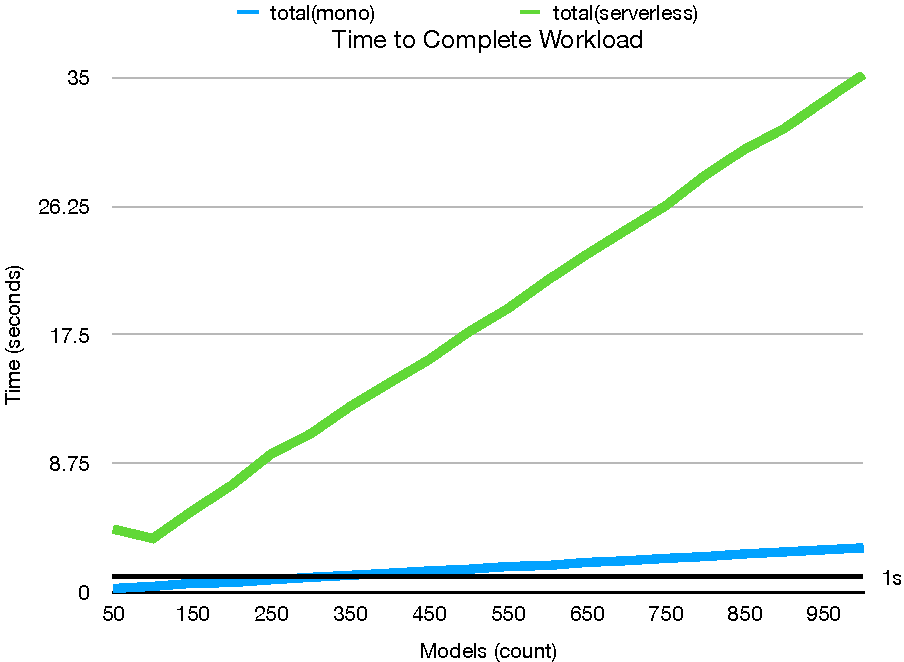
\includegraphics[width=\textwidth]{media/no_rl_ex.pdf}
    \caption{Execution time comparison between serverless and monolithic implementations}
    \label{fig:rate_unlimited_comparison}
\end{figure}
The serverless implementation's execution time increased incomparably to the monolithic version, as seen on figure 5.1.
While for both implementations the median latency did tend to increase, the serverless implementation's latency increased considerably faster, as seen in figures 5.2 and 5.3.
\begin{figure}[h!]
    \centering
    \begin{minipage}{0.48\textwidth}
        \centering
        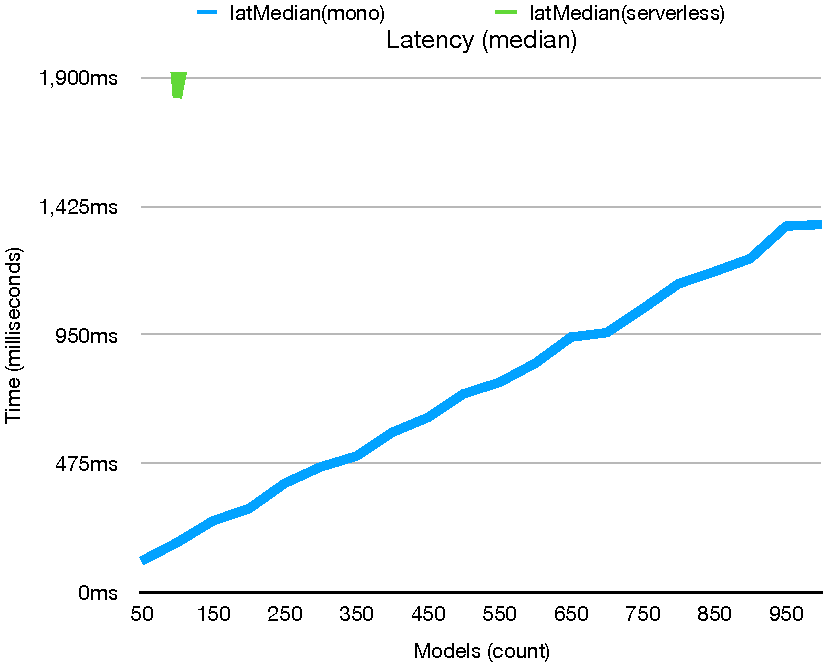
\includegraphics[width=\linewidth]{media/no_rl_mono_lat_med.pdf}
        \caption{Median latency for a single model request, scaled for the monolithic implementation}
        \label{fig:rate_unlimited_comparison_lat_mono}
    \end{minipage}\hfill
    \begin{minipage}{0.48\textwidth}
        \centering
        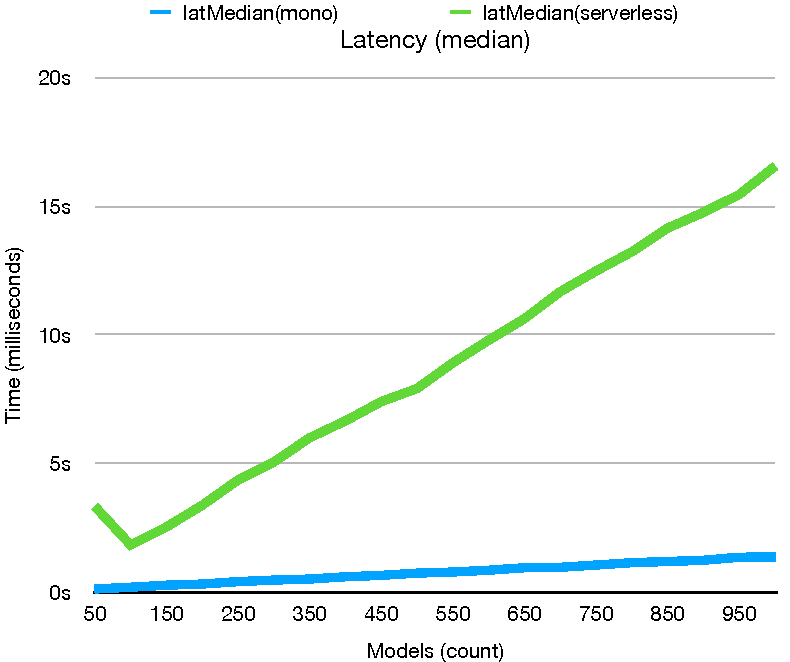
\includegraphics[width=\linewidth]{media/no_rl_lat_med.pdf}
        \caption{Median latency for a single model request}
        \label{fig:rate_unlimited_comparison_lat}
    \end{minipage}
\end{figure}

The above is explained by a much lower Queries per Second (QPS) by the serverless implementation. As seen on figure 5.4, while the serverless implementation seems to have hit a limit of 28 QPS, the serverless implementation seems to hit a limit of 333, more than ten times bigger.
\begin{figure}[h!]
    \centering
    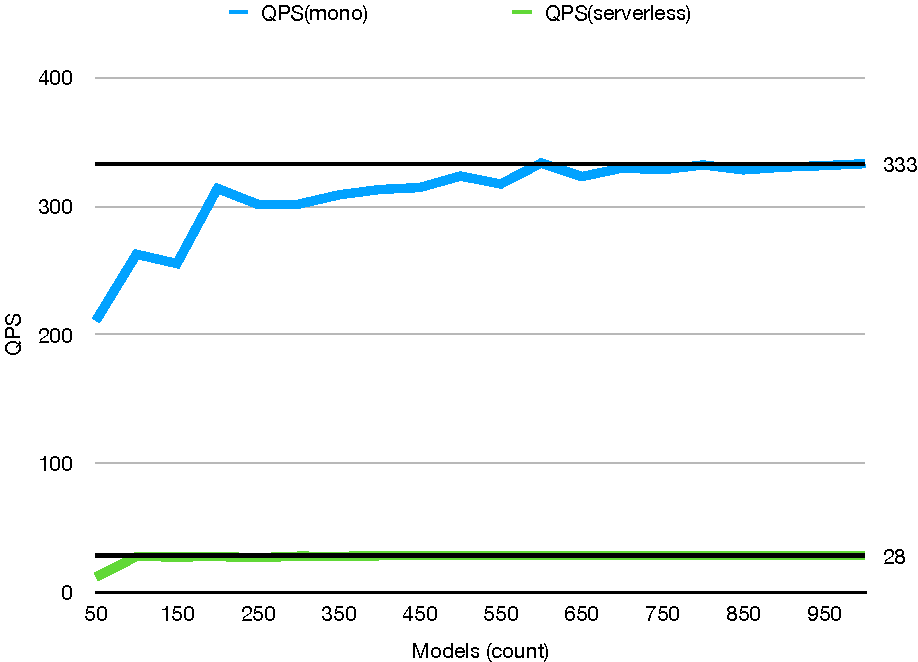
\includegraphics[width=\textwidth]{media/no_rl_qps.pdf}
    \caption{QPS comparison between serverless and monolithic implementations}
    \label{fig:rate_unlimited_comparison_qps}
\end{figure}


\subsection{Implementing a Rate Limit}
We use the Swift Rate Limitter, which is a custom made Swift rate limitter we have developed~\cite{swift-rl}, which is well tested, which allows us to send requests with a minimum set delay between them. We utilized it to send the requests every 100ms. This will cap the maximum QPS to 10 which ensures neither implementation will be stressed, hopefully allowing us to have a clearer picture of the situtation.

With the rate limit both implementations take the same amount of time and bot achieve roughly 10QPS.
As evident from figure 5.5, a single model sync takes roughly 280ms and 60ms on the serverless and monolithic implementations respectively.
\begin{figure}[h!]
    \centering
    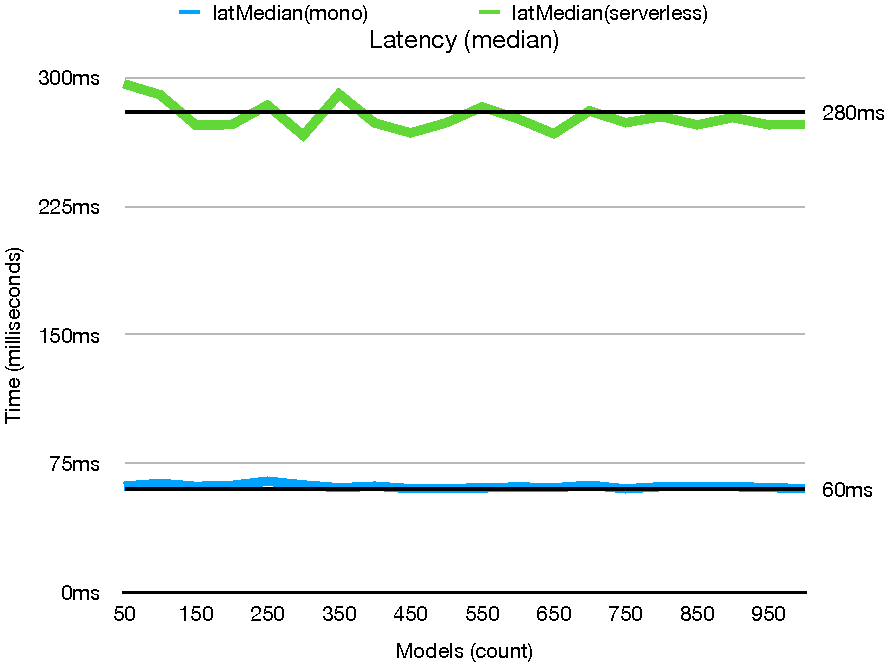
\includegraphics[width=\textwidth]{media/rl100_lat_med.pdf}
    \caption{Rate-limited (100ms) comparison between serverless and monolithic implementations}
    \label{fig:rate_limited_comparison}
\end{figure}
An interesting finding, is that the P99.9\% latency (figures 5.6 and 5.7), apart from being higher, it as less stable on the serverless implementation. This is despite utilizing less than the third of its maximum QPS.
\begin{figure}[h!]
    \centering
    \begin{minipage}{0.48\textwidth}
        \centering
        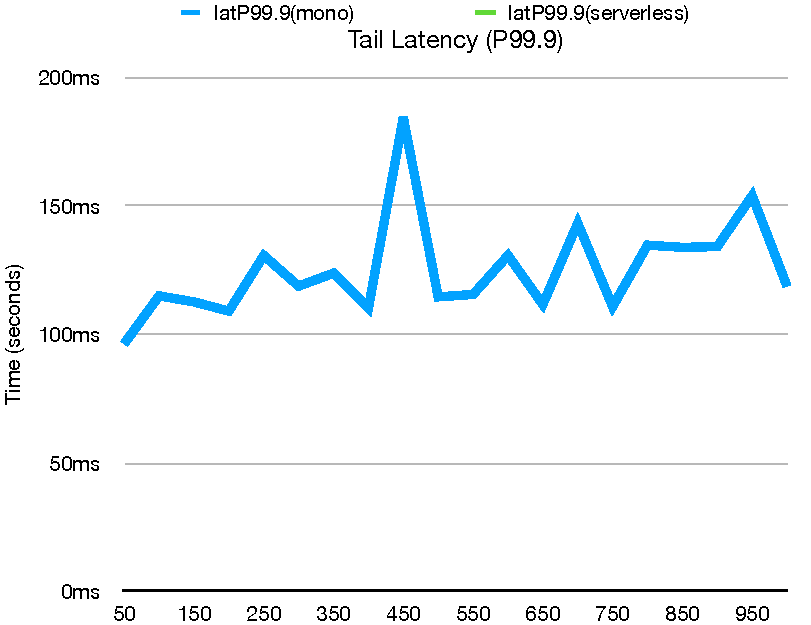
\includegraphics[width=\linewidth]{media/rl100_tl_mono.pdf}
        \caption{Median latency for a single model request, scaled for the monolithic implementation}
        \label{fig:rate_unlimited_comparison_lat_mono}
    \end{minipage}\hfill
    \begin{minipage}{0.48\textwidth}
        \centering
        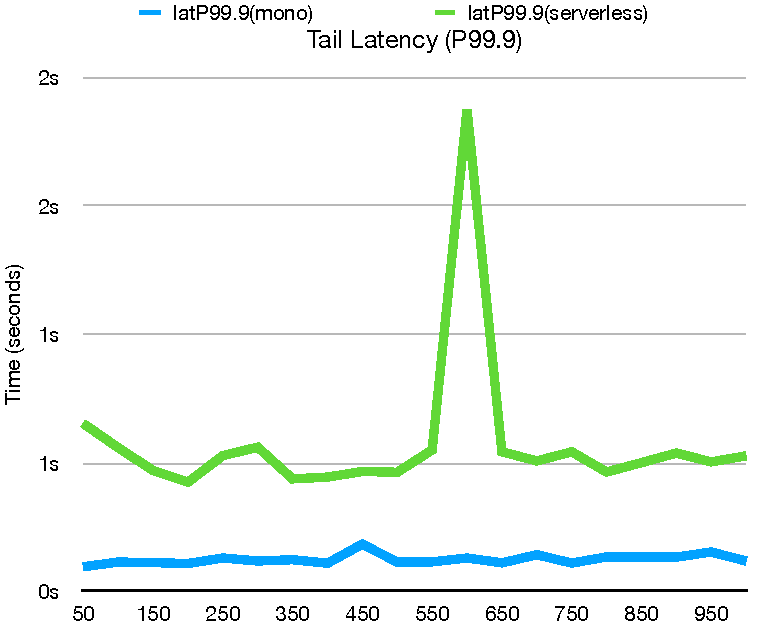
\includegraphics[width=\linewidth]{media/rl100_tl.pdf}
        \caption{Median latency for a single model request}
        \label{fig:rate_unlimited_comparison_lat}
    \end{minipage}
\end{figure}

Despite utilizing 18 machines for executing actions, the serverless approach did not show any clear benefits. This may be attributed to the lack of support for "intra-concurrency" in OpenWhisk runtimes, excluding NodeJS. This limitation significantly affects the scaling capabilities of the serverless implementation, which is a crucial aspect of the serverless or FaaS promise. 18 machines achieving 28QPS means that on average, a request takes 642ms to complete, which is more than double of the 280ms it takes, when the system is not stressed.

\section{Improvements and Future Work}

There are potential avenues for improvement in the serverless system. Notably, updating the Go proxy used by all OpenWhisk runtimes to support intra-concurrency could allow all language runtimes, including Swift, to support concurrent executions, potentially dramatically increasing the maximum QPS.

\section{Conclusion}

The case study findings contribute to the overall conclusion of this thesis, suggesting that the benefit of migrating to a serverless implementation is not always evident and should be carefully assessed for each workflow. The case study also highlights the importance of runtime support for intra-concurrency in realizing the full potential of serverless systems. Without intra-concurrency, the requests stay in memory until a container is available to serve them. The overheads of OpenWhisk may explain the 2 times slowdown of its request completion under load. Notably, the Swift runtime was updated to the latest version to leverage its native async/await features, which played a significant role in the serverless implementation. A total of eighteen identical machines achieving a throughput of ten times less than one single, identical machine is frankly unacceptable. Support for intra-concurrency for the ActionLoop proxy should be a priority for the OpenWhisk project as seamless, efficient scaling is the central promise of FaaS.


